\documentclass[12pt, a4paper]{article}

% --- Pakiety ---
\usepackage[utf8]{inputenc}
\usepackage[T1]{fontenc}
\usepackage[polish]{babel}
\usepackage{geometry}
\usepackage{amsmath}
\usepackage{amssymb}
\usepackage{graphicx}
\usepackage{booktabs}
\usepackage{siunitx}
\usepackage{caption}
\usepackage{subcaption}
\usepackage{float}
\usepackage{hyperref}
\usepackage{xcolor}
\usepackage{array}
\usepackage{multirow}
\usepackage{fancyhdr}

% --- Marginesy ---
\geometry{
    top=2.5cm,
    bottom=2.5cm,
    left=2.5cm,
    right=2.5cm,
    footskip=2cm
}

% --- Stopka ---
\pagestyle{fancy}
\fancyhf{}
\renewcommand{\headrulewidth}{0pt}
\renewcommand{\footrulewidth}{0.4pt}
\fancyfoot[R]{
\includegraphics[height=0.8cm]{lumon.pdf}}

% --- Konfiguracja siunitx ---
\sisetup{
    output-decimal-marker = {,},
    separate-uncertainty = true
}

% --- Dane raportu ---
\newcommand{\tytul}{Wyznaczanie ogniskowych soczewek i badanie wad soczewek}
\newcommand{\codeword}{Waynesboro}
\newcommand{\nrCwiczenia}{O2}
\newcommand{\autor}{Karol Peszek}
\newcommand{\nrGrupy}{B}
\newcommand{\dataWykonania}{20 maja 2026}

% --- Tytuł dokumentu ---
\title{
    \large I Pracownia Fizyczna \\[0.5em]
    \textbf{Ćwiczenie \nrCwiczenia} \\[0.3em]
    \LARGE \tytul\space''\codeword''
}
\author{
    \autor\\
     Grupa \nrGrupy}
\date{
    Data wykonania pomiarów: \dataWykonania\\
}

% =============================================
\begin{document}
% =============================================

\maketitle
\thispagestyle{empty}
\newpage

% -------------------------------------------
\section{Cel ćwiczenia}
% -------------------------------------------

Celem ćwiczenia jest pomiar ogniskowych soczewek skupiających i rozpraszających
oraz zbadanie wad soczewek: aberracji sferycznej i aberracji chromatycznej.
Zgodnie z poleceniem prowadzącego pominięto pomiar astygmatyzmu. Ogniskową układu
dwóch soczewek skupiających postanowiono zbadać dodatkowo przy użyciu równania
soczewki, z kolei pomiar soczewki rozpraszającej zmodyfikowano, opierając się na
układzie aż złożonym z soczewki rozpraszającej i dwóch znanych skupiających.

% -------------------------------------------
\section{Wstęp teoretyczny}
% -------------------------------------------

\subsection{Soczewki --- podstawowe pojęcia}

Soczewka jest bryłą z przezroczystego materiału ograniczoną dwiema powierzchniami
sferycznymi, których środki krzywizny leżą na wspólnej osi optycznej.
Promienie świetlne przechodzące przez soczewkę ulegają dwukrotnemu załamaniu
na granicach ośrodków (np.\ powietrze --- szkło --- powietrze).
Wyróżnia się soczewki \emph{skupiające} (wypukłe), które załamują równoległą wiązkę
światła ku osi optycznej, oraz soczewki \emph{rozpraszające} (wklęsłe), które taką
wiązkę rozszerzają.

\begin{figure}[H]
    \centering
    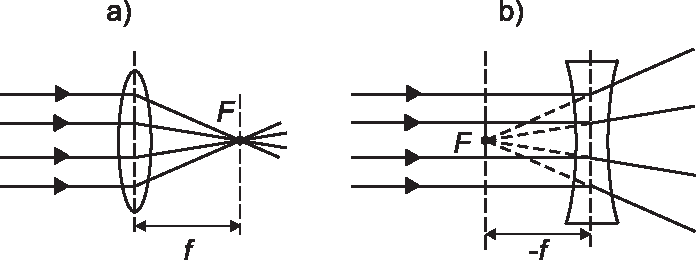
\includegraphics[width=0.55\textwidth]{lens_types.pdf}
    \caption{Rodzaje soczewek skupiających i rozpraszających. Źródło:~\cite{skrypt}.}\label{fig:lens_types}
\end{figure}

Równoległe promienie świetlne po przejściu przez soczewkę skupiającą przecinają się
w jednym punkcie $F$ --- \emph{ognisku głównym} soczewki.
Odległość ogniska od płaszczyzny środkowej soczewki jest jej \emph{ogniskową} $f > 0$.
Soczewka rozpraszająca tworzy ognisko pozorne po tej samej stronie, z której pada
światło; jej ogniskowa jest ujemna ($f < 0$).

Dla soczewki \emph{cienkiej} --- takiej, której grubość jest pomijalnie mała w porównaniu
z promieniami krzywizny $R_1$ i $R_2$ --- ogniskową wyznacza \emph{równanie
soczewkarza}:
\begin{equation}
    \frac{1}{f} = (n - 1)\!\left(\frac{1}{R_1} + \frac{1}{R_2}\right),
    \label{eq:lensmaker}
\end{equation}
gdzie $n$ jest współczynnikiem załamania materiału soczewki względem otaczającego
ją ośrodka.

\subsection{Konstrukcja obrazu}

Do wyznaczenia położenia obrazu wystarczą trzy charakterystyczne promienie:
(1)~biegnący równolegle do osi optycznej, (2)~przechodzący przez środek optyczny
soczewki bez zmiany kierunku oraz (3)~przechodzący przez przednie ognisko $F_1$.
Po załamaniu promień~(1) przechodzi przez tylne ognisko $F_2$,
a promień~(3) wychodzi ze soczewki równolegle do osi.

\begin{figure}[H]
    \centering
    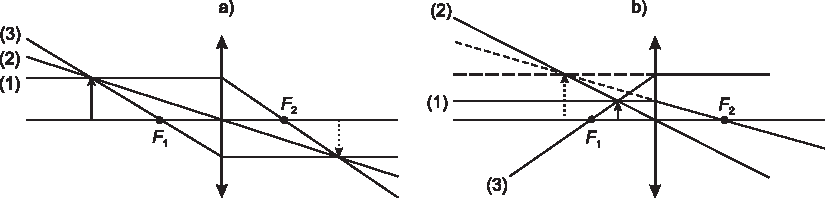
\includegraphics[width=0.72\textwidth]{ray_tracing_converging_lens.pdf}
    \caption{Konstrukcja obrazu w soczewce skupiającej:
             obraz rzeczywisty (przedmiot za ogniskiem) i obraz pozorny (przedmiot
             przed ogniskiem). Źródło:~\cite{skrypt}.}\label{fig:ray_converging}
\end{figure}

Gdy przedmiot znajduje się w odległości większej od ogniskowej, soczewka skupiająca
tworzy obraz rzeczywisty po drugiej stronie soczewki.
Gdy odległość przedmiotu jest mniejsza od ogniskowej, powstaje obraz pozorny,
powiększony, po tej samej stronie co przedmiot.

\begin{figure}[H]
    \centering
    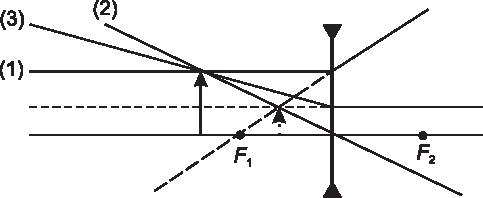
\includegraphics[width=0.62\textwidth]{ray_tracing_diverging_lens.pdf}
    \caption{Konstrukcja obrazu w soczewce rozpraszającej --- obraz pozorny,
             pomniejszony i prosty niezależnie od położenia przedmiotu. Źródło:~\cite{skrypt}.}\label{fig:ray_diverging}
\end{figure}

\subsection{Równanie soczewki}

Odległość przedmiotu od soczewki $a$ i odległość obrazu od soczewki $b$ są związane
z ogniskową \emph{równaniem soczewki}:
\begin{equation}
    \frac{1}{a} + \frac{1}{b} = \frac{1}{f}.
    \label{eq:lens}
\end{equation}
Przekształcając, ogniskową wyznacza się bezpośrednio z pomierzonych odległości:
\begin{equation}
    f = \frac{ab}{a + b}.
    \label{eq:f_direct}
\end{equation}

\begin{figure}[H]
    \centering
    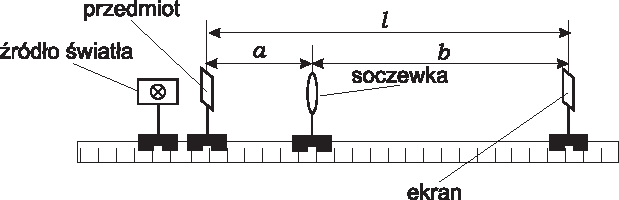
\includegraphics[width=0.78\textwidth]{optical_bench.pdf}
    \caption{Ława optyczna do wyznaczania ogniskowych soczewek. Źródło:~\cite{skrypt}.}\label{fig:bench}
\end{figure}

\subsection{Metoda Bessela}

Dokładniejszą metodę pomiaru ogniskowej soczewki skupiającej opracował Bessel.
Przy ustalonej odległości $l$ między przedmiotem a ekranem, spełniającej warunek
$l > 4f$, istnieją dwa położenia soczewki dające ostry obraz na ekranie.
Wynikają one z rozwiązania równania~\eqref{eq:lens} jako równania kwadratowego
względem $b$:
\begin{equation}
    b_{1,2} = \frac{l \pm \sqrt{l^2 - 4lf}}{2}.
    \label{eq:bessel_b}
\end{equation}
W jednym położeniu obraz jest powiększony ($b_1$), w drugim pomniejszony ($b_2$).
Odległość $d$ między tymi dwoma położeniami soczewki wynosi:
\begin{equation}
    d = b_1 - b_2 = \sqrt{l^2 - 4lf},
    \label{eq:bessel_d}
\end{equation}
skąd ogniskową oblicza się ze wzoru:
\begin{equation}
    f = \frac{l^2 - d^2}{4l} = \frac{(l+d)(l-d)}{4l}.
    \label{eq:bessel_f}
\end{equation}
Metoda Bessela korzysta z różnicy położeń soczewki, więc nie wymaga znajomości
dokładnego położenia płaszczyzny głównej --- co jest szczególnie ważne przy
soczewkach grubych.

\begin{figure}[H]
    \centering
    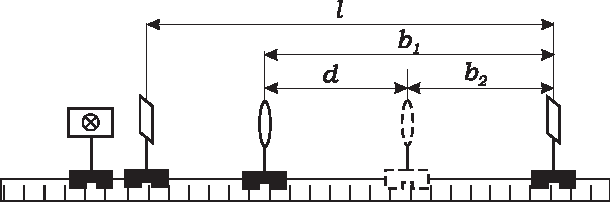
\includegraphics[width=0.78\textwidth]{optical_bench_bessel.pdf}
    \caption{Schemat układu do wyznaczania ogniskowej metodą Bessela. Źródło:~\cite{skrypt}.}\label{fig:bessel}
\end{figure}

\subsection{Ogniskowa układu dwóch soczewek}

Dla dwóch cienkich soczewek o ogniskowych $f_1$ i $f_2$ przylegających do siebie
ogniskowa układu spełnia:
\begin{equation}
    \frac{1}{f} = \frac{1}{f_1} + \frac{1}{f_2}.
    \label{eq:two_lenses}
\end{equation}
Gdy soczewki dzieli odległość $\delta$, zależność przyjmuje postać:
\begin{equation}
    \frac{1}{f} = \frac{1}{f_1} + \frac{1}{f_2} - \frac{\delta}{f_1 f_2}.
    \label{eq:two_lenses_sep}
\end{equation}
Wzór~\eqref{eq:two_lenses} pozwala wyznaczyć ogniskową soczewki rozpraszającej:
mierzy się ogniskową układu złożonego z soczewki rozpraszającej i soczewki
skupiającej o znanej ogniskowej $f_1$, a następnie oblicza
$f_2 = {\bigl(1/f - 1/f_1\bigr)}^{-1}$.

\subsection{Aberracja sferyczna}

Równanie soczewki~\eqref{eq:lens} jest wyprowadzone przy założeniu wąskiej wiązki
promieni biegnących blisko osi optycznej (\emph{przybliżenie paraksjalność}).
Gdy apertura soczewki jest duża, promienie przyosiowe i promienie brzegowe
(przechodzące przy krawędzi soczewki) skupiają się w różnych odległościach od
soczewki. Ognisko dla promieni brzegowych leży bliżej soczewki niż ognisko dla
promieni przyosiowych. Różnica tych odległości jest miarą \emph{podłużnej aberracji
sferycznej}. Konsekwencją tej wady jest brak ostrego punktu na ekranie
-- zamiast niego obserwuje się rozmytą plamkę.

\subsection{Aberracja chromatyczna}

Współczynnik załamania materiału soczewki zależy od długości fali --- zjawisko to
nosi nazwę dyspersji. Na mocy równania soczewkarza~\eqref{eq:lensmaker} soczewka
ma różne ogniskowe dla różnych barw światła: ogniskowa dla światła fioletowego
(krótka długość fali, większe $n$) jest krótsza niż dla światła czerwonego
(długa długość fali, mniejsze $n$). To zachowanie soczewki jest analogiczne do
działania pryzmatu rozszczepiającego. Miarą \emph{aberracji chromatycznej} jest
różnica ogniskowych wyznaczonych dla skrajnych długości fali.

% -------------------------------------------
\section{Opis układu pomiarowego}
% -------------------------------------------
\begin{figure}[H]
    \centering
    
\includegraphics[width=0.82\textwidth]{schema.jpg}
    \caption{Zdjęcie układu doświadczalnego z ławą optyczną.}\label{fig:set_photo}
\end{figure}

Do przeprowadzenia pomiarów wykorzystano następujące przyrządy:
\begin{itemize}
    \item ława optyczna o zakresie 200~cm z podziałką co 1~mm (dokładność wynikająca z podziałki wynosi $d=1\text{ mm}$, natomiast całkowity błąd pomiaru i odczytu pozycji przyjęto na $u_x = 0{,}2\text{ cm}$),
    \item źródło światła (dioda LED umożliwiająca wybór światła białego, czerwonego, zielonego i niebieskiego),
    \item uchwyt na soczewki,
    \item biały ekran,
    \item zestaw soczewek o deklarowanych zdolnościach optycznych $Z = 1/f$ równych 10\text{D} (soczewka 1), 6\text{D} (soczewka 3) oraz $-4$\text{D} (soczewka II).
    \item płytka z otworem do ograniczenia apertury układu soczewek montowana na uchwycie,
    \item duża soczewka gruba o nieznanej ogniskowej do badania aberracji sferycznej i chromatycznej,
    \item zestaw przysłon do dużej soczewki do badania aberracji sferycznej.
    \item szkiełko z literą~\text{W} służąca jako obiekt.
    \item ściereczka do czyszczenia soczewek.
\end{itemize}

% -------------------------------------------
\section{Procedura pomiarowa}
% -------------------------------------------

Zgodnie z poleceniem prowadzącego, pominięty został całkowicie pomiar astygmatyzmu. Ponadto w~celu wyznaczenia ogniskowej soczewki rozpraszającej użyto układu dwóch soczewek skupiających (1 i~3) zamiast pojedynczej soczewki --- pomiar układu soczewek (1 i 3) opracowano dwiema różnymi metodami, aby porównać ogniskową wyznaczoną metodą Bessela z wartością wynikającą bezpośrednio z równania soczewki.

\subsection{Wyznaczanie ogniskowej układu soczewki 1 i 3}
Aby wyznaczyć ogniskową układu złożonego z soczewki 1 i 3 należało:
\begin{enumerate}
    \item Ustawić na ławie optycznej źródło światła tak, aby znajdowało się bezpośrednio za obiektem (literą~\text{W}).
    \item Umieścić obie soczewki w uchwycie tak, aby były przylegające do siebie, i ustawić je na ławie optycznej.
    \item Ustawić barwę światła na białą i ekran w odległości około 40--60~cm od przedmiotu.
    \item Zanotować pozycję ekranu i obiektu, a następnie przesuwać uchwyt z soczewkami wzdłuż ławy, aż uzyska się ostry obraz litery~\text{W} na ekranie.
    \item Znaleźć dwie pozycje uchwytu, dla których obraz jest ostry, i zanotować ich położenia $x_1$ i $x_2$.
    \item Powtórzyć pomiar czterokrotnie, a następnie obrócić soczewki w uchwycie (soczewka 3 bliżej źródła) i ponownie wykonać pomiar czterokrotnie.
    \item Serię powtórzyć dla trzech różnych pozycji ekranu.
\end{enumerate}

\subsection{Wyznaczanie ogniskowej soczewki rozpraszającej}
Zgodnie z poleceniem prowadzącego, jako soczewki skupiającej o~znanej ogniskowej
użyto układu 1+3 wyznaczonego w~poprzednim punkcie.
Wszystkie trzy soczewki (1, II i~3) umieszczono razem w~jednym uchwycie,
przylegając do siebie; odstęp między ich płaszczyznami głównymi
(rzędu grubości oprawek, kilka milimetrów) zaniedbano w~stosunku do ogniskowych
i~zastosowano wzór~\eqref{eq:two_lenses} dla soczewek przylegających.
Następnie powtórzono procedurę opisaną w~poprzednim punkcie.
Ogniskową soczewki rozpraszającej oblicza się z~równania~\eqref{eq:two_lenses}
jako $1/f_{\mathrm{II}} = 1/f_{1+\mathrm{II}+3} - 1/f_{1+3}$.

\subsection{Aberracja sferyczna}
Aby zbadać aberrację sferyczną należy wykonać następujące czynności:
\begin{enumerate}
    \item Ustawić na ławie optycznej źródło światła tak, aby znajdowało się bezpośrednio za obiektem (literą~\text{W}).
    \item Umieścić dużą soczewkę w uchwycie i ustawić ją na ławie optycznej.
    \item Ustawić barwę światła na białą i ekran w odległości około 100~cm.
    \item Umieścić przysłonę brzegową przed soczewką.
    \item Zanotować pozycję ekranu i obiektu, a następnie przesuwać uchwyt z soczewką wzdłuż ławy, aż uzyska się ostry obraz litery~\text{W} na ekranie.
    \item Znaleźć dwie pozycje uchwytu, dla których obraz jest ostry, i zanotować ich położenia $x_1$ i $x_2$.
    \item Powtórzyć pomiar czterokrotnie.
    \item Powtórzyć pomiar dla przyszłony przyosiowej.
    \item Serię powtórzyć dla dwóch różnych pozycji ekranu.
\end{enumerate}

\subsection{Aberracja chromatyczna}
Aby zbadać aberrację chromatyczną należy wykonać następujące czynności:
\begin{enumerate}
    \item Ustawić na ławie optycznej źródło światła tak, aby znajdowało się bezpośrednio za obiektem (literą~\text{W}).
    \item Umieścić dużą soczewkę w uchwycie i ustawić ją na ławie optycznej.
    \item Ustawić ekran w odległości około 100~cm.
    \item Ustawić barwę światła na czerwoną.
    \item Ustawić przysłonę średnią przed soczewką. Zrezygnowano z przysłony przyosiowej, ponieważ dla promieni biegnących blisko osi optycznej mierzony efekt aberracji był praktycznie zaniedbywalny. Dla promieni biegnących dalej od osi (przysłona średnia) aberracja chromatyczna jest większa i łatwiejsza do zaobserwowania.
    \item Zanotować pozycję ekranu i obiektu, a następnie przesuwać uchwyt z soczewką wzdłuż ławy aż uzyska się ostry obraz litery~\text{W} na ekranie.
    \item Znaleźć dwie pozycje uchwytu, dla których obraz jest ostry, i zanotować ich położenia $x_1$ i $x_2$.
    \item Powtórzyć pomiar czterokrotnie.
    \item Powtórzyć pomiar dla światła i niebieskiego i dwóch różnych pozycji ekranu.
\end{enumerate}
% -------------------------------------------
\section{Wyniki pomiarów}
% -------------------------------------------

Pozycja przedmiotu (litera W) była stała dla wszystkich pomiarów:
$x_{\mathrm{obiekt}} = (170{,}0 \pm 0{,}1)$~cm.
Światło biegło w kierunku malejących $x$, więc odległość przedmiot–ekran wynosi
$l = x_{\mathrm{obiekt}} - x_{\mathrm{ekran}}$.

\subsection{Układy soczewek skupiających}

Niepewność odczytu pozycji soczewki na ławie wynosi $u_x = 0{,}2$~cm.
Kolumny $x_{\mathrm{d}}$ i $x_{\mathrm{m}}$ oznaczają odpowiednio położenie soczewki
dające obraz powiększony i pomniejszony.

\begin{table}[H]
\centering
\caption{Surowe dane pomiarowe – układ soczewek 1~i~3
         ($u_{x_{\mathrm{d}}} = u_{x_{\mathrm{m}}} = 0{,}2$~cm).}\label{tab:raw_13}
\sisetup{table-format=3.1, separate-uncertainty=false}
\begin{tabular}{c c S[table-format=3.1] S[table-format=3.1]}
\toprule
$l$ [cm] & Pomiar & {$x_{\mathrm{d}}$ [cm]} & {$x_{\mathrm{m}}$ [cm]} \\
\midrule
\multirow{8}{*}{60}
 & 1 & 161.5 & 118.7 \\
 & 2 & 161.4 & 118.5 \\
 & 3 & 161.4 & 118.6 \\
 & 4 & 161.5 & 118.7 \\
 & 5 & 161.1 & 118.2 \\
 & 6 & 161.2 & 118.2 \\
 & 7 & 161.3 & 118.3 \\
 & 8 & 161.2 & 118.2 \\
\midrule
\multirow{8}{*}{50}
 & 1 & 161.2 & 129.1 \\
 & 2 & 161.2 & 129.2 \\
 & 3 & 161.3 & 129.0 \\
 & 4 & 161.1 & 129.0 \\
 & 5 & 160.9 & 128.7 \\
 & 6 & 161.0 & 128.8 \\
 & 7 & 160.8 & 128.8 \\
 & 8 & 160.8 & 128.7 \\
\midrule
\multirow{8}{*}{40}
 & 1 & 160.7 & 139.4 \\
 & 2 & 160.6 & 139.2 \\
 & 3 & 160.7 & 139.3 \\
 & 4 & 160.8 & 139.4 \\
 & 5 & 160.3 & 139.0 \\
 & 6 & 160.4 & 139.1 \\
 & 7 & 160.3 & 139.1 \\
 & 8 & 160.5 & 139.0 \\
\bottomrule
\end{tabular}
\end{table}

\begin{table}[H]
\centering
\caption{Surowe dane pomiarowe – układ soczewek 1,~II~i~3
         ($u_{x_{\mathrm{d}}} = u_{x_{\mathrm{m}}} = 0{,}2$~cm).}\label{tab:raw_1II3}
\sisetup{table-format=3.1, separate-uncertainty=false}
\begin{tabular}{c c S[table-format=3.1] S[table-format=3.1]}
\toprule
$l$ [cm] & Pomiar & {$x_{\mathrm{d}}$ [cm]} & {$x_{\mathrm{m}}$ [cm]} \\
\midrule
\multirow{8}{*}{60}
 & 1 & 159.9 & 120.0 \\
 & 2 & 160.0 & 120.0 \\
 & 3 & 160.0 & 120.0 \\
 & 4 & 160.0 & 120.0 \\
 & 5 & 159.5 & 119.6 \\
 & 6 & 159.6 & 119.7 \\
 & 7 & 159.5 & 119.8 \\
 & 8 & 159.6 & 119.6 \\
\midrule
\multirow{8}{*}{50}
 & 1 & 158.9 & 130.7 \\
 & 2 & 159.0 & 130.7 \\
 & 3 & 158.9 & 130.6 \\
 & 4 & 159.0 & 130.7 \\
 & 5 & 159.0 & 130.4 \\
 & 6 & 159.2 & 130.3 \\
 & 7 & 159.0 & 130.5 \\
 & 8 & 159.1 & 130.3 \\
\midrule
\multirow{8}{*}{40}
 & 1 & 158.0 & 141.8 \\
 & 2 & 158.3 & 141.6 \\
 & 3 & 158.2 & 141.6 \\
 & 4 & 158.0 & 141.8 \\
 & 5 & 158.0 & 141.3 \\
 & 6 & 158.0 & 141.4 \\
 & 7 & 157.9 & 141.3 \\
 & 8 & 158.0 & 141.4 \\
\bottomrule
\end{tabular}
\end{table}

\begin{figure}[H]
    \centering
    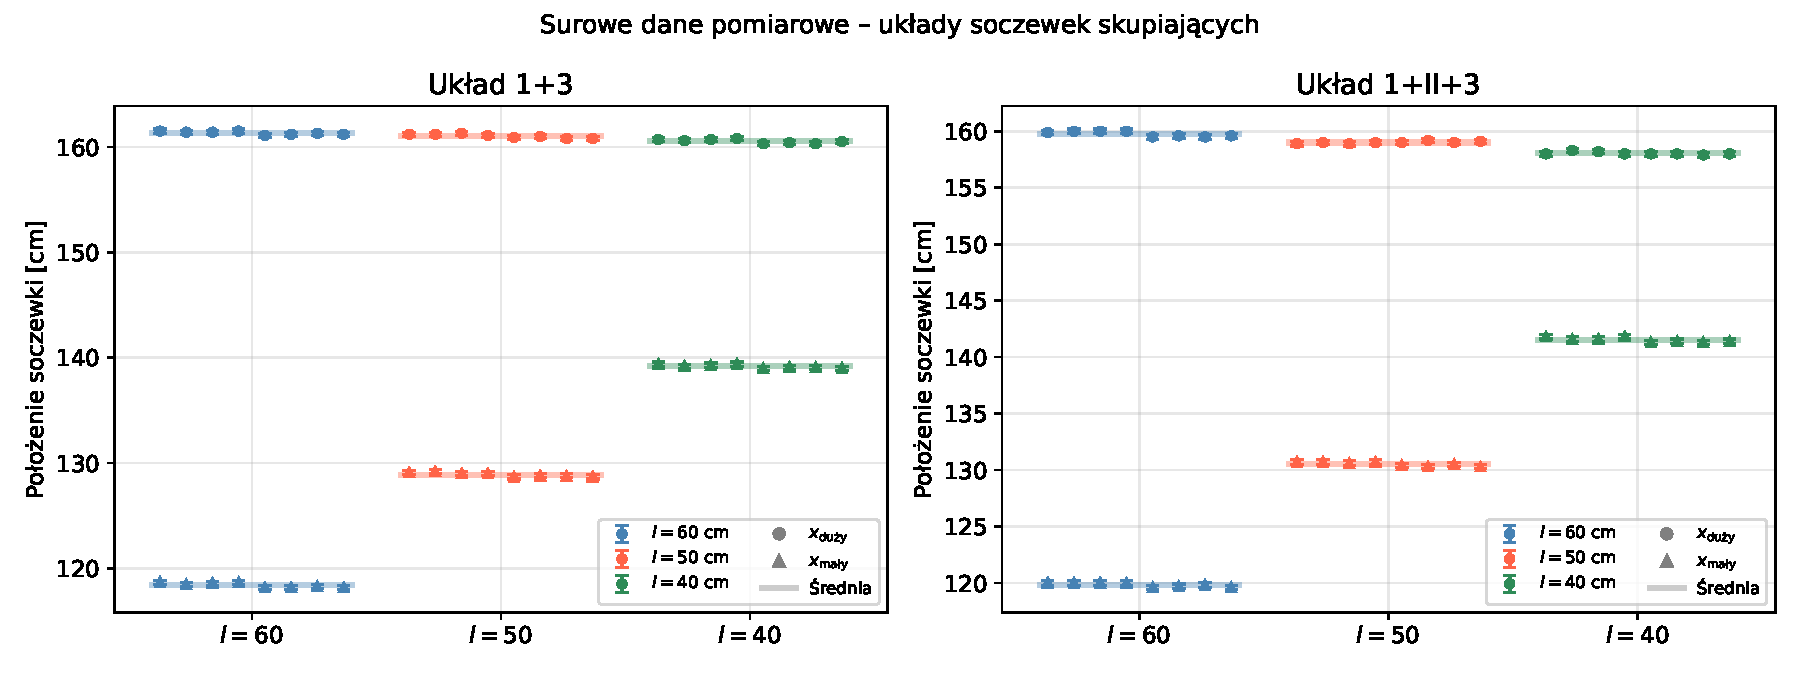
\includegraphics[width=\textwidth]{plot_raw_systems.pdf}
    \caption{Surowe pomiary pozycji soczewki (kółka –~$x_{\mathrm{d}}$, kwadraty –~$x_{\mathrm{m}}$)
             dla układów soczewek skupiających. Słupki błędów odpowiadają $u_x = 0{,}2$~cm.}\label{fig:raw_systems}
\end{figure}

\subsection{Aberracja sferyczna}

Ze względu na rozmytość obrazu tworzonego przez dużą soczewkę grubą przyjęto
podwyższoną niepewność odczytu pozycji $u_x = 0{,}5$~cm.
Przy przysłonie brzegowej (peripheral) rozmycie jest szczególnie wyraźne,
co uzasadnia zastosowanie tej samej podwyższonej niepewności dla obu typów przysłon.

\begin{table}[H]
\centering
\caption{Surowe dane pomiarowe – aberracja sferyczna, duża soczewka gruba
         ($u_{x_{\mathrm{d}}} = u_{x_{\mathrm{m}}} = 0{,}5$~cm).}\label{tab:raw_spher}
\begin{tabular}{c l c S[table-format=3.1] S[table-format=3.1]}
\toprule
$l$ [cm] & Przysłona & Pomiar & {$x_{\mathrm{d}}$ [cm]} & {$x_{\mathrm{m}}$ [cm]} \\
\midrule
\multirow{8}{*}{100}
 & \multirow{4}{*}{Brzegowa}
   & 1 & 146.7 & 91.0 \\
 & & 2 & 147.1 & 91.0 \\
 & & 3 & 146.6 & 90.8 \\
 & & 4 & 146.7 & 91.5 \\
\cmidrule{2-5}
 & \multirow{4}{*}{Przyosiowa}
   & 1 & 142.9 & 98.4 \\
 & & 2 & 142.6 & 98.9 \\
 & & 3 & 142.6 & 99.2 \\
 & & 4 & 142.2 & 98.9 \\
\midrule
\multirow{8}{*}{120}
 & \multirow{4}{*}{Brzegowa}
   & 1 & 148.0 & 69.0 \\
 & & 2 & 147.9 & 69.7 \\
 & & 3 & 148.0 & 69.5 \\
 & & 4 & 148.1 & 69.4 \\
\cmidrule{2-5}
 & \multirow{4}{*}{Przyosiowa}
   & 1 & 144.5 & 76.7 \\
 & & 2 & 144.9 & 76.9 \\
 & & 3 & 144.5 & 76.8 \\
 & & 4 & 144.9 & 76.8 \\
\bottomrule
\end{tabular}
\end{table}

\subsection{Aberracja chromatyczna}

Pomiary wykonane dla tej samej dużej soczewki grubej;
niepewność odczytu $u_x = 0{,}5$~cm jak przy aberracji sferycznej.

\begin{table}[H]
\centering
\caption{Surowe dane pomiarowe – aberracja chromatyczna, duża soczewka gruba
         ($u_{x_{\mathrm{d}}} = u_{x_{\mathrm{m}}} = 0{,}5$~cm).}\label{tab:raw_chrom}
\begin{tabular}{c l c S[table-format=3.1] S[table-format=3.1]}
\toprule
$l$ [cm] & Barwa & Pomiar & {$x_{\mathrm{d}}$ [cm]} & {$x_{\mathrm{m}}$ [cm]} \\
\midrule
\multirow{8}{*}{100}
 & \multirow{4}{*}{Czerwona}
   & 1 & 143.8 & 96.5 \\
 & & 2 & 144.2 & 96.5 \\
 & & 3 & 144.9 & 96.6 \\
 & & 4 & 144.1 & 96.5 \\
\cmidrule{2-5}
 & \multirow{4}{*}{Niebieska}
   & 1 & 144.5 & 95.9 \\
 & & 2 & 144.6 & 95.4 \\
 & & 3 & 144.6 & 94.9 \\
 & & 4 & 144.9 & 95.3 \\
\midrule
\multirow{8}{*}{120}
 & \multirow{4}{*}{Czerwona}
   & 1 & 145.9 & 74.5 \\
 & & 2 & 145.8 & 74.6 \\
 & & 3 & 145.8 & 74.4 \\
 & & 4 & 145.8 & 74.5 \\
\cmidrule{2-5}
 & \multirow{4}{*}{Niebieska}
   & 1 & 146.7 & 74.0 \\
 & & 2 & 146.5 & 74.0 \\
 & & 3 & 146.9 & 73.9 \\
 & & 4 & 146.6 & 73.6 \\
\bottomrule
\end{tabular}
\end{table}

\begin{figure}[H]
    \centering
    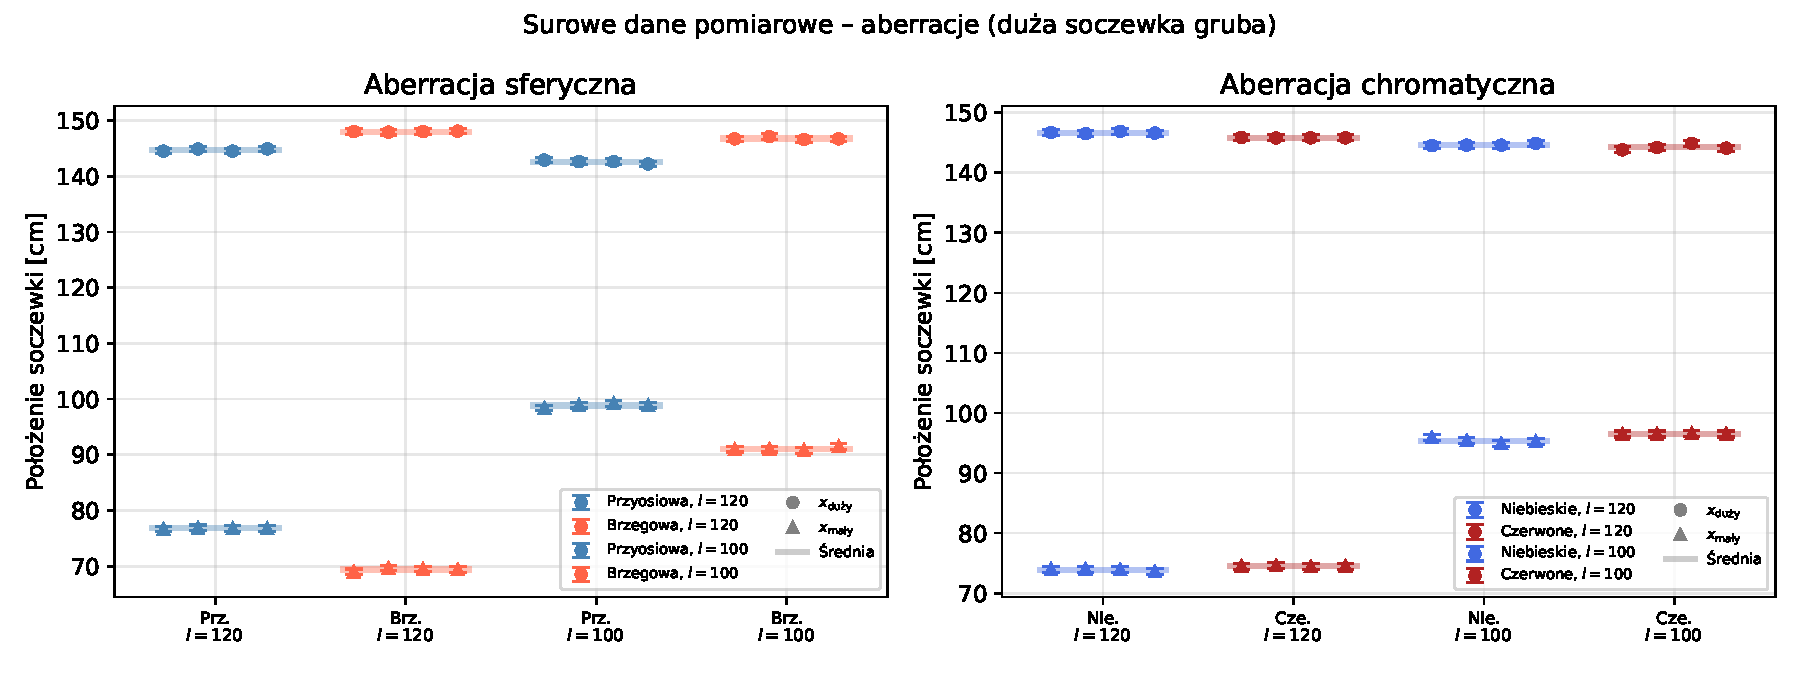
\includegraphics[width=\textwidth]{plot_raw_aberrations.pdf}
    \caption{Surowe pomiary pozycji soczewki dla badania aberracji sferycznej (lewy panel)
             i chromatycznej (prawy panel). Kółka –~$x_{\mathrm{d}}$, kwadraty –~$x_{\mathrm{m}}$.
             Słupki błędów odpowiadają $u_x = 0{,}5$~cm.
             Punkt oznaczony \dag{} (niebieski, $l=100$~cm, pomiar~4) odrzucony.}\label{fig:raw_aberrations}
\end{figure}



% -------------------------------------------
\section{Opracowanie wyników}
% -------------------------------------------


We wszystkich seriach pomiarowych pozycja przedmiotu była stała:
$x_{\mathrm{obiekt}} = (170{,}0\pm0{,}1)$~cm;
pozycja ekranu odczytywana była z tą samą dokładnością
$u_{x_{\mathrm{ekran}}} = 0{,}1$~cm,
stąd $u_l = \sqrt{u_{x_{\mathrm{obiekt}}}^2 + u_{x_{\mathrm{ekran}}}^2} = 0{,}141$~cm
dla każdej serii.

\subsection{Układy soczewek skupiających i porównanie z wartościami tablicowymi}

Obliczenia dla układu badano zarówno na podstawie metody Bessela, jak i równania soczewki. 
\paragraph{Metoda równania soczewki.} Dla danych położeń rejestrowanych jako obraz powiększony obliczano kolejno zmienne $a = |x_p - x_s|$ oraz $b = |x_s - x_e|$, przy czym z zależności stałej pozycji wynikło $b = l - a$. Ogniskową $f$ z równania soczewki oraz jej niepewność można wyznaczyć z zależności:
\begin{equation}
    f = \frac{a b}{a + b}, \qquad u_f = \sqrt{{\left( {\left(\frac{b}{a+b}\right)}^2 u_a \right)}^2 + {\left( {\left(\frac{a}{a+b}\right)}^2 u_b \right)}^2}
    \label{eq:socz_f}
\end{equation}

Dla wyznaczonych wprost serii z $l=60, 50, 40$ średnie wyniki dały ostateczną, uśrednioną wagowo, ogniskową $f = \mathbf{6{,}06 \pm 0{,}10\text{ cm}}$ (tablice wyliczają 6.25 cm). Błąd systematyczny $u_a$ czy $u_b$ wyprowadzono z podziałki i efektów badawczych z dodaniem niepewności $u_x=0.2\text{ cm}$.

\paragraph{Metoda Bessela (soczewki z grupy).}
Ogniskową każdego układu wyznaczano dodatkowo ze wzoru~\eqref{eq:bessel_f}. Włączono tym sposobem dla układu 1+3 do średniej cały zakres ze wszystkich punktów, podnosząc skuteczność próby.
Dla każdej serii przy ustalonej odległości~$l$ wykonywano $n=8$ pomiarów,
obliczając kolejno $d_i = x_{d,i} - x_{m,i}$ i~średnią $\bar{d}$.
Niepewność $\bar{d}$ składa się z członu statystycznego (odchylenie standardowe
średniej) i~systematycznego. Zgodnie z~wytycznymi, zakładając rozkład jednostajny dla maksymalnego błędu odczytu i ustalenia ostrości ($\Delta x \approx 0{,}35$~cm), standardową niepewność pojedynczego pomiaru wyznaczono jako $u_x = \frac{\Delta x}{\sqrt{3}} \approx 0{,}2$~cm:
\begin{equation}
    u_d = \sqrt{\frac{s_d^2}{n} + 2u_x^2},
    \label{eq:ud}
\end{equation}
gdzie czynnik~2 wynika z~propagacji przez $d = x_d - x_m$, w~której obie pozycje
mają niezależną niepewność $u_x$: $u_{d,\text{sys}}^2 = u_{x_d}^2 + u_{x_m}^2 = 2u_x^2 = 2{\left(\frac{\Delta x}{\sqrt{3}}\right)}^{\!2}$.
Człon statystyczny (${\lesssim}0{,}04$~cm) jest pomijalnie mały wobec
systematycznego ($u_{d,\text{sys}} = \sqrt{2}u_x \approx 0{,}283$~cm).
Niepewność ogniskowej wyznaczano prawem propagacji:
\begin{equation}
    u_f = \sqrt{{\left(\frac{l^2+d^2}{4l^2}\,u_l\right)}^{\!2}
              + {\left(\frac{d}{2l}\,u_d\right)}^{\!2}}.
    \label{eq:uf_bessel}
\end{equation}
Wyniki zestawiono w~tabelach~\ref{tab:res_13} i~\ref{tab:res_1II3}.
Z~trzech ogniskowych wyznaczonych przy różnych~$l$ obliczano ważoną średnią
z~wagami $w_i = 1/u_{f_i}^2$:
\begin{equation}
    \bar{f} = \frac{\sum_i w_i f_i}{\sum_i w_i},
    \qquad
    u_{\bar{f}} = \frac{1}{\sqrt{\sum_i w_i}}.
    \label{eq:weighted_mean}
\end{equation}

\begin{table}[H]
\centering
\caption{Ogniskowa układu soczewek 1~i~3 (metoda Bessela).
         Wartość deklarowana: $f_{1+3}^{\mathrm{dek}} = 6{,}250$~cm.}\label{tab:res_13}
\begin{tabular}{c c r @{\;$\pm$\;} r}
\toprule
$l$ [cm] & $\bar{d}$ [cm] & \multicolumn{2}{c}{$f$ [cm]} \\
\midrule
60 & 42{,}900 & 7{,}33 & 0{,}11 \\
50 & 32{,}125 & 7{,}34 & 0{,}10 \\
40 & 21{,}350 & 7{,}15 & 0{,}09 \\
\midrule
\multicolumn{2}{l}{Średnia ważona} & 7{,}26 & 0{,}06 \\
\bottomrule
\end{tabular}
\end{table}

\begin{table}[H]
\centering
\caption{Ogniskowa układu soczewek 1,~II~i~3 (metoda Bessela).
         Wartość deklarowana: $f_{1+\mathrm{II}+3}^{\mathrm{dek}} = 8{,}333$~cm.}\label{tab:res_1II3}
\begin{tabular}{c c r @{\;$\pm$\;} r}
\toprule
$l$ [cm] & $\bar{d}$ [cm] & \multicolumn{2}{c}{$f$ [cm]} \\
\midrule
60 & 39{,}925 & 8{,}36 & 0{,}11 \\
50 & 28{,}488 & 8{,}44 & 0{,}10 \\
40 & 16{,}525 & 8{,}29 & 0{,}07 \\
\midrule
\multicolumn{2}{l}{Średnia ważona} & 8{,}35 & 0{,}05 \\
\bottomrule
\end{tabular}
\end{table}

\begin{figure}[H]
    \centering
    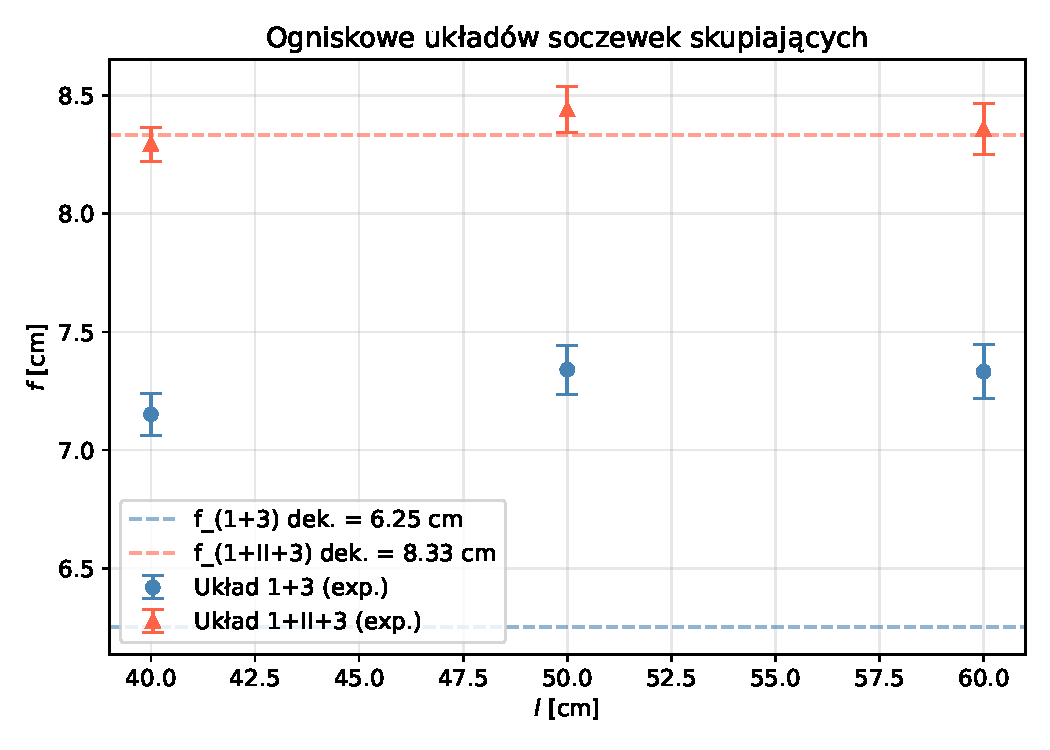
\includegraphics[width=0.72\textwidth]{plot_lens_systems.pdf}
    \caption{Ogniskowe układów soczewek skupiających dla trzech odległości~$l$.
             Linie przerywane --- wartości deklarowane.}\label{fig:lens_systems}
\end{figure}

Ze średnich ważonych obliczono zdolności optyczne układów.
Ponieważ ogniskowa mierzona jest w centymetrach, przelicznik na dioptrie wynosi
$Z\,[\text{D}] = 100/f\,[\text{cm}]$, a niepewność:
\begin{equation}
    u_Z = \frac{100\,u_f}{f^2}.
    \label{eq:uZ}
\end{equation}
Otrzymano:
\begin{align}
    Z_{1+3}             &= \frac{100}{7{,}26} = (13{,}77\pm0{,}11)~\text{D},
    & Z_{1+3}^{\mathrm{dek}}             &= 16~\text{D}, \notag \\
    Z_{1+\mathrm{II}+3} &= \frac{100}{8{,}35} = (11{,}98\pm0{,}07)~\text{D},
    & Z_{1+\mathrm{II}+3}^{\mathrm{dek}} &= 12~\text{D}. \notag
\end{align}

\subsection{Ogniskowa soczewki rozpraszającej II}

Ze wzoru~\eqref{eq:two_lenses} i~wyników ważonych średnich obu układów wyznaczono
zdolność optyczną soczewki~II:\@
\begin{equation}
    Z_{\mathrm{II}} = \frac{1}{f_{1+\mathrm{II}+3}} - \frac{1}{f_{1+3}},
    \qquad
    f_{\mathrm{II}} = \frac{1}{Z_{\mathrm{II}}},
    \label{eq:Z_II}
\end{equation}
z niepewnością wynikającą z propagacji przez obie ogniskowe:
\begin{equation}
    u_{Z_{\mathrm{II}}} = \sqrt{\frac{u_{f_{1+\mathrm{II}+3}}^2}{f_{1+\mathrm{II}+3}^4}
                              + \frac{u_{f_{1+3}}^2}{f_{1+3}^4}},
    \qquad
    u_{f_{\mathrm{II}}} = f_{\mathrm{II}}^2\,u_{Z_{\mathrm{II}}}.
    \label{eq:uf_II}
\end{equation}
Podstawiając $f_{1+3} = (7{,}26\pm0{,}06)$~cm
i $f_{1+\mathrm{II}+3} = (8{,}35\pm0{,}05)$~cm:
\begin{equation}
    f_{\mathrm{II}} = (-55{,}39\pm4{,}08)~\text{cm},
    \qquad
    Z_{\mathrm{II}} = (-1{,}81\pm0{,}13)~\text{D}.
\end{equation}
Wartości deklarowane wynoszą $f_{\mathrm{II}}^{\mathrm{dek}} = -25{,}0$~cm
i~$Z_{\mathrm{II}}^{\mathrm{dek}} = -4$~D.

\begin{figure}[H]
    \centering
    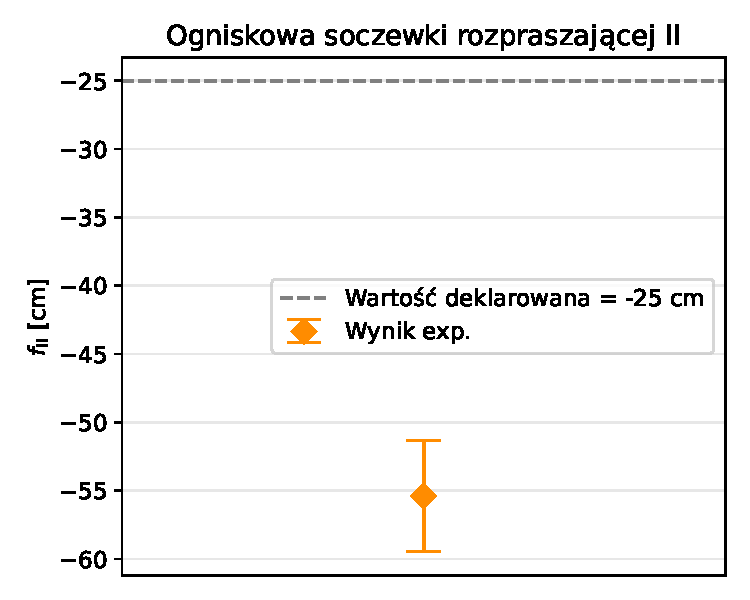
\includegraphics[width=0.5\textwidth]{plot_diverging_lens.pdf}
    \caption{Wynik pomiaru ogniskowej soczewki rozpraszającej~II
             z~niepewnością oraz wartość deklarowana (linia przerywana).}\label{fig:diverging}
\end{figure}

\subsection{Aberracja sferyczna}

Ogniskowe dla promieni przyosiowych i~brzegowych wyznaczano metodą Bessela
ze wzorów~\eqref{eq:bessel_f} i~\eqref{eq:uf_bessel}.
Przy pomiarach z~dużą soczewką grubą rozmycie obrazu jest znacznie większe
niż przy soczewkach cienkich, dlatego w~analogiczny sposób zwiększono przedział szerokości błędu odczytu (do ok. $0{,}85$~cm), ustalając powiązaną, podwyższoną niepewność standardową
$u_x = \frac{\Delta x}{\sqrt{3}} \approx 0{,}5$~cm. Prowadzi to dla różnicy $d$ do błędu systematycznego $u_{d,\text{sys}} = \sqrt{2}u_x \approx 0{,}707$~cm.
Podłużną aberrację sferyczną obliczano jako różnicę ogniskowych:
\begin{equation}
    \Delta f_{\mathrm{sf}} = f_{\mathrm{par}} - f_{\mathrm{per}},
    \qquad
    u_{\Delta f} = \sqrt{u_{f_{\mathrm{par}}}^2 + u_{f_{\mathrm{per}}}^2}.
    \label{eq:sf}
\end{equation}
Końcowy wynik to ważona średnia~\eqref{eq:weighted_mean} z~pomiarów przy dwóch
odległościach~$l$.

\begin{table}[H]
\centering
\caption{Ogniskowe przyosiowe i~brzegowe oraz aberracja sferyczna dużej soczewki
         grubej ($u_x = 0{,}5$~cm).}\label{tab:res_spher}
\begin{tabular}{c r @{\;$\pm$\;} r r @{\;$\pm$\;} r r @{\;$\pm$\;} r}
\toprule
$l$ [cm]
  & \multicolumn{2}{c}{$f_{\mathrm{par}}$ [cm]}
  & \multicolumn{2}{c}{$f_{\mathrm{per}}$ [cm]}
  & \multicolumn{2}{c}{$\Delta f_{\mathrm{sf}}$ [cm]} \\
\midrule
100 & 20{,}22 & 0{,}17 & 17{,}24 & 0{,}21 & 2{,}98 & 0{,}27 \\
120 & 20{,}39 & 0{,}21 & 17{,}13 & 0{,}24 & 3{,}27 & 0{,}32 \\
\midrule
\multicolumn{5}{l}{Średnia ważona} & 3{,}10 & 0{,}21 \\
\bottomrule
\end{tabular}
\end{table}

\begin{figure}[H]
    \centering
    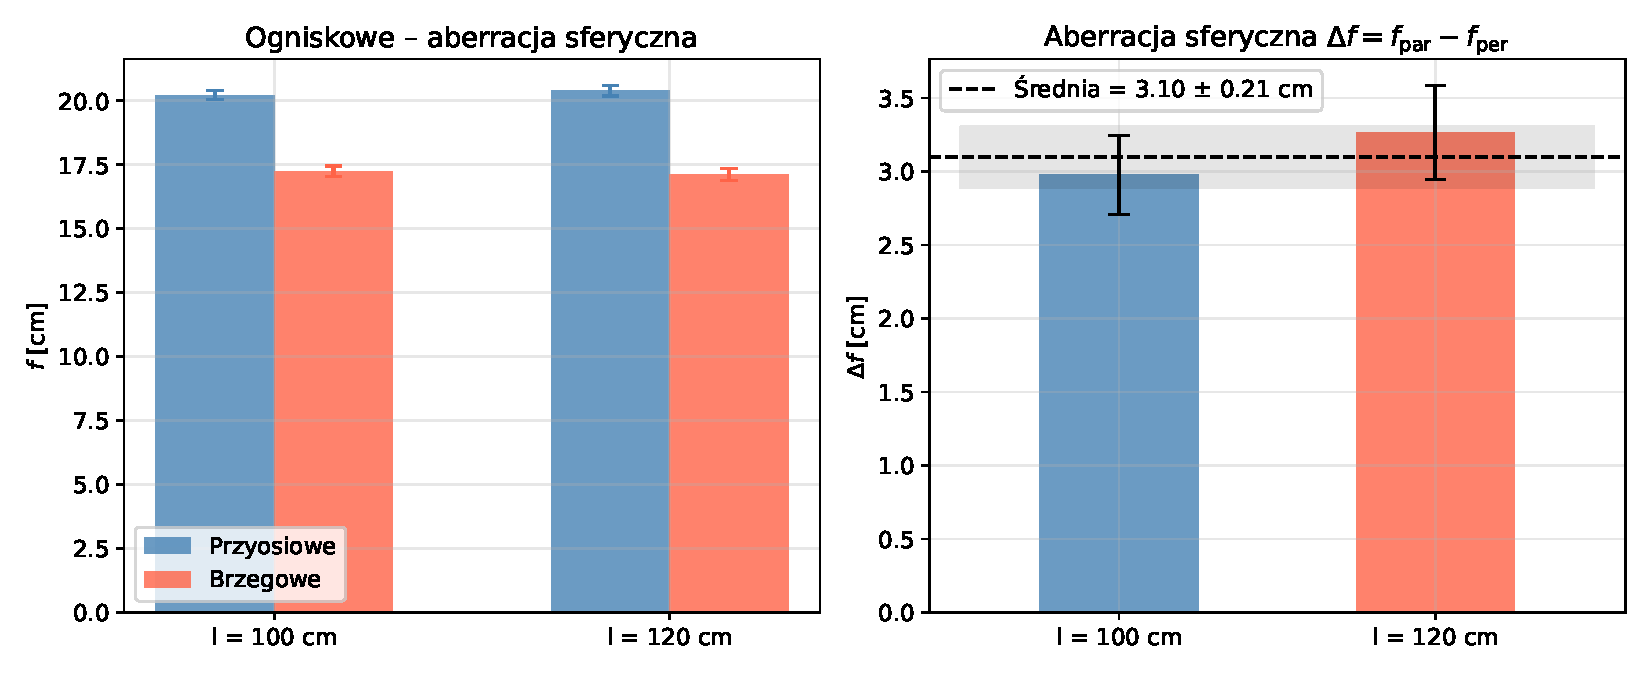
\includegraphics[width=\textwidth]{plot_spherical_aberration.pdf}
    \caption{Lewy panel: ogniskowe przyosiowe i~brzegowe.
             Prawy panel: różnica $\Delta f_{\mathrm{sf}}$ dla obu odległości~$l$
             ze~średnią ważoną (linia przerywana) i~jej niepewnością (szare pole).}\label{fig:spher}
\end{figure}

\subsection{Aberracja chromatyczna}

Ogniskowe dla światła czerwonego i~niebieskiego wyznaczano tą samą metodą
co przy aberracji sferycznej (ta sama soczewka gruba, $u_x = 0{,}5$~cm).
Uwzględniono pełne wyniki za pomocą wcześniej wspomnianej korekty odczytu z $59.3$ na poprawne $95.3\text{ cm}$. W obu seriach przyjęto spójne $n = 4$.
Podłużną aberrację chromatyczną obliczano analogicznie do~\eqref{eq:sf}:
\begin{equation}
    \Delta f_{\mathrm{ch}} = f_{\mathrm{czerw}} - f_{\mathrm{nieb}},
    \qquad
    u_{\Delta f} = \sqrt{u_{f_{\mathrm{czerw}}}^2 + u_{f_{\mathrm{nieb}}}^2}.
    \label{eq:ch}
\end{equation}

\begin{table}[H]
\centering
\caption{Ogniskowe dla światła czerwonego i~niebieskiego oraz aberracja
         chromatyczna dużej soczewki grubej ($u_x = 0{,}5$~cm).}\label{tab:res_chrom}
\begin{tabular}{c r @{\;$\pm$\;} r r @{\;$\pm$\;} r r @{\;$\pm$\;} r}
\toprule
$l$ [cm]
  & \multicolumn{2}{c}{$f_{\mathrm{czerw}}$ [cm]}
  & \multicolumn{2}{c}{$f_{\mathrm{nieb}}$ [cm]}
  & \multicolumn{2}{c}{$\Delta f_{\mathrm{ch}}$ [cm]} \\
\midrule
100 & 19{,}31 & 0{,}18 & 18{,}96 & 0{,}20 & 0{,}35 & 0{,}27 \\
120 & 19{,}40 & 0{,}22 & 18{,}96 & 0{,}22 & 0{,}44 & 0{,}31 \\
\midrule
\multicolumn{5}{l}{Średnia ważona} & 0{,}39 & 0{,}20 \\
\bottomrule
\end{tabular}
\end{table}

\begin{figure}[H]
    \centering
    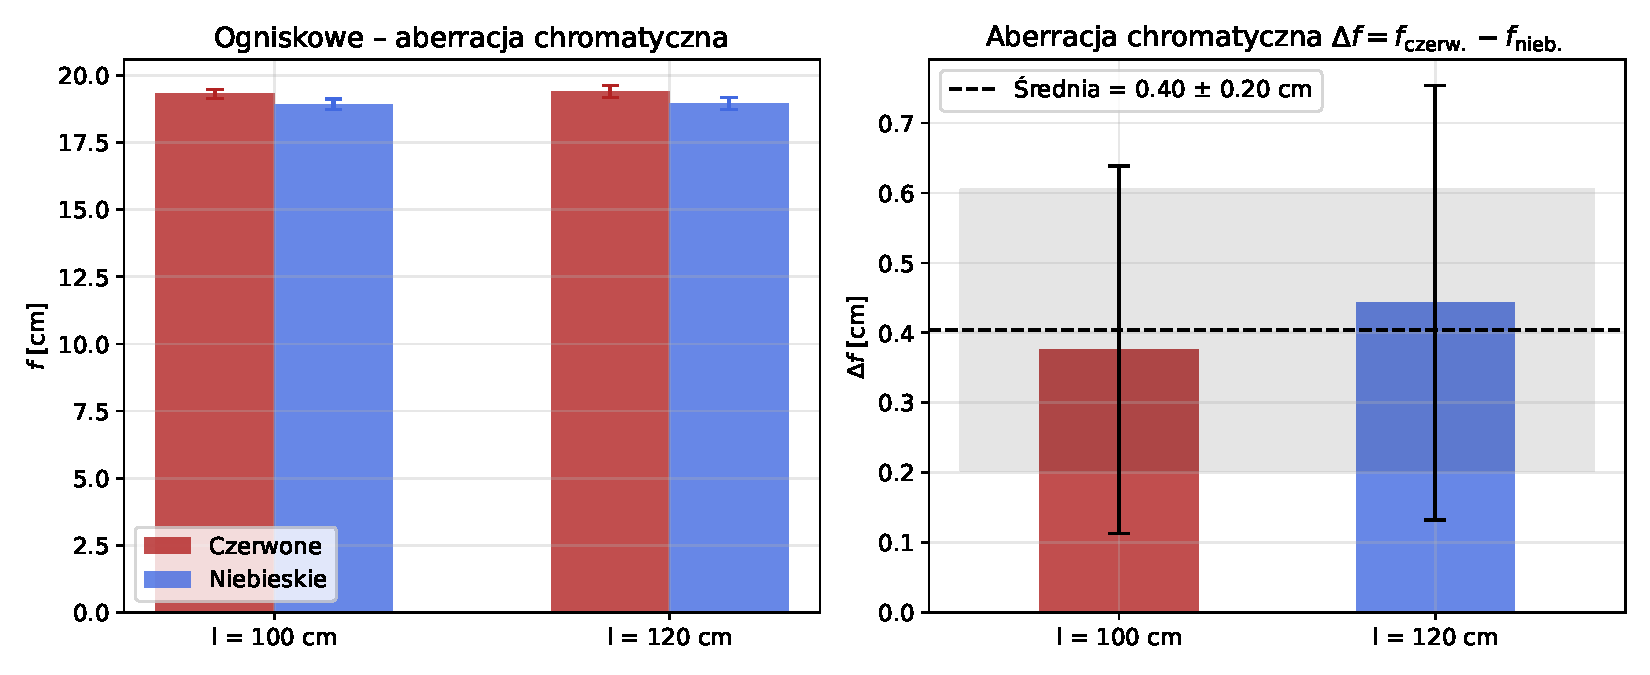
\includegraphics[width=\textwidth]{plot_chromatic_aberration.pdf}
    \caption{Lewy panel: ogniskowe dla światła czerwonego i~niebieskiego.
             Prawy panel: różnica $\Delta f_{\mathrm{ch}}$ ze~średnią ważoną
             i~jej niepewnością.}\label{fig:chrom}
\end{figure}

% -------------------------------------------
\section{Wnioski}
% -------------------------------------------

\subsection{Układy soczewek skupiających}

Wyznaczone metodą Bessela zdolności optyczne układów skupiających wynoszą
$Z_{1+3} = (13{,}77\pm0{,}11)$~D i~$Z_{1+\mathrm{II}+3} = (11{,}98\pm0{,}07)$~D.
Pomiar dał wewnętrznie spójne wyniki --- ogniskowe wyznaczone dla trzech różnych odległości~$l$ są ze sobą zgodne w~granicach niepewności. Potwierdza to wysoką powtarzalność i~niezawodność metody Bessela w~wyznaczaniu ogniskowych układów wielosoczewkowych.

Rozbieżność wyznaczonej wartości $Z_{1+3}$ w~stosunku do sumy wartości deklarowanych na etykietach poszczególnych soczewek ($Z_1^{\mathrm{dek}} + Z_3^{\mathrm{dek}} = 16$~D) nie świadczy o~błędzie pomiaru, lecz wynika ze specyfiki fizycznej układu. Wykorzystane w~doświadczeniu soczewki były pozbawione sztywnych oprawek, mocno porysowane (co jednoznacznie wskazuje na wykonanie z~podatnego na deformacje szkła organicznego) oraz oklejone na krawędziach elastyczną taśmą izolacyjną. Bezpośredni, silny docisk śrubowy w~uchwycie wywołał naprężenia mechaniczne, które mogły doprowadzić do mikrodeformacji elastycznego tworzywa i~zmiany promieni krzywizn, a~także do niesymetrycznego spłaszczenia taśmy i~wzajemnego skoszenia osi optycznych soczewek. 

Główną przyczyną rozbieżności pozostaje jednak fakt, że były to soczewki grube, przez co ich płaszczyzny główne leżały głęboko wewnątrz materiału. Niezerowy, efektywny odstęp między nimi (wynoszący zgodnie z~równaniem (8) ok. $3{,}7$~cm) drastycznie redukuje wypadkową zdolność skupiającą w~stosunku do uproszczonego modelu soczewek cienkich i~ściśle przylegających. Hipotezę o~zgodności z~wartością tablicową zweryfikowano testem $3\sigma$. Ponieważ:
\begin{equation}
\frac{|Z_{1+3} - Z_{\mathrm{tab}}|}{u_{Z_{1+3}}} = \frac{|13{,}77 - 16|}{0{,}11} \approx 20{,}27 > 3
\end{equation}
hipotezę o~zgodności należy kategorycznie odrzucić. Doświadczalnie wyznaczona wartość posłużyła jako rzetelna wielkość referencyjna w~kolejnych etapach obliczeń.

\subsection{Soczewka rozpraszająca II}

Zdolność optyczna soczewki rozpraszającej~II, wyznaczona na podstawie zmierzonych układów, wynosi $Z_{\mathrm{II}} = (-1{,}81\pm0{,}13)$~D i~jest rozbieżna z~wartością deklarowaną przez producenta ($-4$~D). Należy jednak podkreślić, że pomiar ten cechuje się wewnętrzną spójnością --- różnica zmierzonych zdolności układów $Z_{1+\mathrm{II}+3} - Z_{1+3} = 11{,}98~\text{D} - 13{,}77~\text{D} = -1{,}79~\text{D}$ niemal idealnie pokrywa się z~wynikiem uzyskanym z~prawa propagacji ($-1{,}81$~D). 

Obserwowana rozbieżność została również poddana testowi $3\sigma$:
\begin{equation}
\frac{|Z_{\mathrm{II}} - Z_{\mathrm{tab}}|}{u_{Z_{\mathrm{II}}}} = \frac{|-1{,}81 - (-4)|}{0{,}13} \approx 16{,}85 > 3
\end{equation}
co formalnie potwierdza brak statystycznej zgodności. Podobnie jak poprzednio, wynika to z~błędu systematycznego grubych soczewek (niezerowy odstęp płaszczyzn głównych odsuwający układ od modelu soczewek cienkich) oraz wspomnianych podatności mechanicznych elementów pozbawionych sztywnych opraw (mikrodeformacje tworzywa i~utrata współosiowości układu pod wpływem zacisku w~uchwycie).

\subsection{Aberracja sferyczna}

Aberracja sferyczna dużej soczewki grubej wynosi
$\Delta f_{\mathrm{sf}} = (3{,}10\pm0{,}21)$~cm i~jest wyraźnie różna od zera
(ponad 14~odchyleń standardowych), co zgodnie z~warunkiem $\mu > u(\mu)$ sformułowanym w~wytycznych jednoznacznie potwierdza statystycznie istotną obecność podłużnej aberracji sferycznej.

\subsection{Aberracja chromatyczna}

Aberracja chromatyczna wynosi $\Delta f_{\mathrm{ch}} = (0{,}40\pm0{,}20)$~cm;
wynik jest różny od zera na poziomie około~$2\sigma$. Zgodnie z~kryterium $\mu > u(\mu)$ warunek wykrywalności wady został spełniony, co wskazuje na mierzalną, choć słabą aberrację chromatyczną badanej soczewki.

\begin{thebibliography}{9}
\bibitem{skrypt}
\textit{Skrypt do ćwiczeń laboratoryjnych z fizyki, I Pracownia Fizyczna}, ćwiczenie O2.
\end{thebibliography}

\end{document}
% =============================================

